\chapter{Classes and objects}

Code examples from this chapter are available from
\url{http://thinkpython.com/code/Point1.py}; solutions
to the exercises are available from
\url{http://thinkpython.com/code/Point1_soln.py}.


\section{User-defined types}
\label{point}
\index{user-defined type}
\index{type!user-defined}

We have used many of Python's built-in types; now we are going
to define a new type.  As an example, we will create a type
called {\tt Point} that represents a point in two-dimensional
space.
\index{point, mathematical}

In mathematical notation, points are often written in
parentheses with a comma separating the coordinates. For example,
$(0,0)$ represents the origin, and $(x,y)$ represents the
point $x$ units to the right and $y$ units up from the origin.

There are several ways we might represent points in Python:

\begin{itemize}

\item We could store the coordinates separately in two
variables, {\tt x} and {\tt y}.

\item We could store the coordinates as elements in a list
or tuple.

\item We could create a new type to represent points as
objects.

\end{itemize}
\index{representation}

Creating a new type
is (a little) more complicated than the other options, but
it has advantages that will be apparent soon.

A user-defined type is also called a {\bf class}.
A class definition looks like this:
\index{class}
\index{object}
\index{class definition}
\index{definition!class}

\begin{verbatim}
class Point(object):
    """Represents a point in 2-D space."""
\end{verbatim}
%
This header indicates that the new class is a {\tt Point},
which is a kind of {\tt object}, which is a built-in
type.
\index{Point class}
\index{class!Point}

The body is a docstring that explains what the class is for.
You can define variables and functions inside a class definition,
but we will get back to that later.
\index{docstring}

Defining a class named {\tt Point} creates a class object.

\begin{verbatim}
>>> print Point
<class '__main__.Point'>
\end{verbatim}
%
Because {\tt Point} is defined at the top level, its ``full
name'' is \verb"__main__.Point".
\index{object!class}
\index{class object}

The class object is like a factory for creating objects.  To create a
Point, you call {\tt Point} as if it were a function.

\begin{verbatim}
>>> blank = Point()
>>> print blank
<__main__.Point instance at 0xb7e9d3ac>
\end{verbatim}
%
The return value is a reference to a Point object, which we
assign to {\tt blank}.  
Creating a new object is called
{\bf instantiation}, and the object is an {\bf instance} of
the class.
\index{instance}
\index{instantiation}

When you print an instance, Python tells you what class it
belongs to and where it is stored in memory (the prefix
{\tt 0x} means that the following number is in hexadecimal).
\index{hexadecimal}


\section{Attributes}
\label{attributes}
\index{instance attribute}
\index{attribute!instance}
\index{dot notation}

You can assign values to an instance using dot notation:

\begin{verbatim}
>>> blank.x = 3.0
>>> blank.y = 4.0
\end{verbatim}
%
This syntax is similar to the syntax for selecting a variable from a
module, such as {\tt math.pi} or {\tt string.whitespace}.  In this case,
though, we are assigning values to named elements of an object.
These elements are called {\bf attributes}.

As a noun, ``AT-trib-ute'' is pronounced with emphasis on the first
syllable, as opposed to ``a-TRIB-ute,'' which is a verb.

The following diagram shows the result of these assignments.
A state diagram that shows an object and its attributes is
called an {\bf object diagram}; see Figure~\ref{fig.point}.
\index{state diagram}
\index{diagram!state}
\index{object diagram}
\index{diagram!object}

\begin{figure}
\centerline
{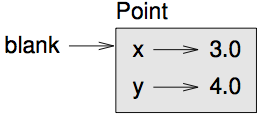
\includegraphics[scale=0.8]{figs/point.pdf}}
\caption{Object diagram.}
\label{fig.point}
\end{figure}


The variable {\tt blank} refers to a Point object, which
contains two attributes.  Each attribute refers to a
floating-point number.

You can read the value of an attribute using the same syntax:

\begin{verbatim}
>>> print blank.y
4.0
>>> x = blank.x
>>> print x
3.0
\end{verbatim}
%
The expression {\tt blank.x} means, ``Go to the object {\tt blank}
refers to and get the value of {\tt x}.'' In this case, we assign that
value to a variable named {\tt x}.  There is no conflict between
the variable {\tt x} and the attribute {\tt x}.

You can use dot notation as part of any expression.  For example:

\begin{verbatim}
>>> print '(%g, %g)' % (blank.x, blank.y)
(3.0, 4.0)
>>> distance = math.sqrt(blank.x**2 + blank.y**2)
>>> print distance
5.0
\end{verbatim}
%
You can pass an instance as an argument in the usual way.
For example:
\index{instance!as argument}

\begin{verbatim}
def print_point(p):
    print '(%g, %g)' % (p.x, p.y)
\end{verbatim}
%
\verb"print_point" takes a point as an argument and displays it in
mathematical notation.  To invoke it, you can pass {\tt blank} as
an argument:

\begin{verbatim}
>>> print_point(blank)
(3.0, 4.0)
\end{verbatim}
%
Inside the function, {\tt p} is an alias for {\tt blank}, so if
the function modifies {\tt p}, {\tt blank} changes.
\index{aliasing}


\begin{exercise}

Write a function called \verb"distance_between_points" that takes two
Points as arguments and returns the distance between them.

\end{exercise}



\section{Rectangles}
\label{rectangles}

Sometimes it is obvious what the attributes of an object should be,
but other times you have to make decisions.  For example, imagine you
are designing a class to represent rectangles.  What attributes would
you use to specify the location and size of a rectangle?  You can
ignore angle; to keep things simple, assume that the rectangle is
either vertical or horizontal.
\index{representation}

There are at least two possibilities: 

\begin{itemize}

\item You could specify one corner of the rectangle
(or the center), the width, and the height.

\item You could specify two opposing corners.

\end{itemize}

At this point it is hard to say whether either is better than
the other, so we'll implement the first one, just as an example.
\index{Rectangle class}
\index{class!Rectangle}

Here is the class definition:

\begin{verbatim}
class Rectangle(object):
    """Represents a rectangle. 

    attributes: width, height, corner.
    """
\end{verbatim}
%
The docstring lists the attributes:  {\tt width} and
{\tt height} are numbers; {\tt corner} is a Point object that
specifies the lower-left corner.

To represent a rectangle, you have to instantiate a Rectangle
object and assign values to the attributes:

\begin{verbatim}
box = Rectangle()
box.width = 100.0
box.height = 200.0
box.corner = Point()
box.corner.x = 0.0
box.corner.y = 0.0
\end{verbatim}
%
The expression {\tt box.corner.x} means,
``Go to the object {\tt box} refers to and select the attribute named
{\tt corner}; then go to that object and select the attribute named
{\tt x}.''

\begin{figure}
\centerline
{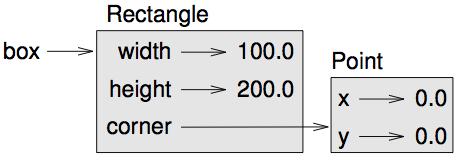
\includegraphics[scale=0.8]{figs/rectangle.pdf}}
\caption{Object diagram.}
\label{fig.rectangle}
\end{figure}


Figure~\ref{fig.rectangle} shows the state of this object.
\index{state diagram}
\index{diagram!state}
\index{object diagram}
\index{diagram!object}
An object that is an attribute of another object is {\bf embedded}.
\index{embedded object}
\index{object!embedded}


\section{Instances as return values}
\index{instance!as return value}
\index{return value}

Functions can return instances.  For example, \verb"find_center"
takes a {\tt Rectangle} as an argument and returns a {\tt Point}
that contains the coordinates of the center of the {\tt Rectangle}:

\begin{verbatim}
def find_center(rect):
    p = Point()
    p.x = rect.corner.x + rect.width/2.0
    p.y = rect.corner.y + rect.height/2.0
    return p
\end{verbatim}
%
Here is an example that passes {\tt box} as an argument and assigns
the resulting Point to {\tt center}:

\begin{verbatim}
>>> center = find_center(box)
>>> print_point(center)
(50.0, 100.0)
\end{verbatim}
%

\section{Objects are mutable}
\index{object!mutable}
\index{mutability}

You can change the state of an object by making an assignment to one of
its attributes.  For example, to change the size of a rectangle
without changing its position, you can modify the values of {\tt
width} and {\tt height}:

\begin{verbatim}
box.width = box.width + 50
box.height = box.width + 100
\end{verbatim}
%
You can also write functions that modify objects.  For example,
\verb"grow_rectangle" takes a Rectangle object and two numbers,
{\tt dwidth} and {\tt dheight}, and adds the numbers to the
width and height of the rectangle:

\begin{verbatim}
def grow_rectangle(rect, dwidth, dheight):
    rect.width += dwidth
    rect.height += dheight
\end{verbatim}
%
Here is an example that demonstrates the effect:

\begin{verbatim}
>>> print box.width
100.0
>>> print box.height
200.0
>>> grow_rectangle(box, 50, 100)
>>> print box.width
150.0
>>> print box.height
300.0
\end{verbatim}
%
Inside the function, {\tt rect} is an
alias for {\tt box}, so if the function modifies {\tt rect}, 
{\tt box} changes.

\begin{exercise}

Write a function named \verb"move_rectangle" that takes
a Rectangle and two numbers named {\tt dx} and {\tt dy}.  It
should change the location of the rectangle by adding {\tt dx}
to the {\tt x} coordinate of {\tt corner} and adding {\tt dy}
to the {\tt y} coordinate of {\tt corner}.

\end{exercise}


\section{Copying}
\label{copying}
\index{aliasing}

Aliasing can make a program difficult to read because changes
in one place might have unexpected effects in another place.
It is hard to keep track of all the variables that might refer
to a given object.
\index{copying objects}
\index{object!copying}
\index{copy module}
\index{module!copy}

Copying an object is often an alternative to aliasing.
The {\tt copy} module contains a function called {\tt copy} that
can duplicate any object:

\begin{verbatim}
>>> p1 = Point()
>>> p1.x = 3.0
>>> p1.y = 4.0

>>> import copy
>>> p2 = copy.copy(p1)
\end{verbatim}
%
{\tt p1} and {\tt p2} contain the same data, but they are
not the same Point.

\begin{verbatim}
>>> print_point(p1)
(3.0, 4.0)
>>> print_point(p2)
(3.0, 4.0)
>>> p1 is p2
False
>>> p1 == p2
False
\end{verbatim}
%
The {\tt is} operator indicates that {\tt p1} and {\tt p2} are not the
same object, which is what we expected.  But you might have expected
{\tt ==} to yield {\tt True} because these points contain the same
data.  In that case, you will be disappointed to learn that for
instances, the default behavior of the {\tt ==} operator is the same
as the {\tt is} operator; it checks object identity, not object
equivalence.  This behavior can be changed---we'll see how later.
\index{is operator}
\index{operator!is}

If you use {\tt copy.copy} to duplicate a Rectangle, you will find
that it copies the Rectangle object but not the embedded Point.
\index{embedded object!copying}

\begin{verbatim}
>>> box2 = copy.copy(box)
>>> box2 is box
False
>>> box2.corner is box.corner
True
\end{verbatim}

\begin{figure}
\centerline
{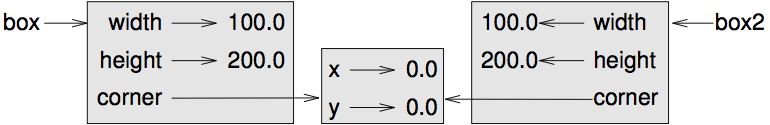
\includegraphics[scale=0.8]{figs/rectangle2.pdf}}
\caption{Object diagram.}
\label{fig.rectangle2}
\end{figure}

Figure~\ref{fig.rectangle2} shows what the object diagram looks like.
\index{state diagram}
\index{diagram!state}
\index{object diagram}
\index{diagram!object}
This operation is called a {\bf shallow copy} because it copies the
object and any references it contains, but not the embedded objects.
\index{shallow copy}
\index{copy!shallow}

For most applications, this is not what you want.  In this example,
invoking \verb"grow_rectangle" on one of the Rectangles would not
affect the other, but invoking \verb"move_rectangle" on either would
affect both!  This behavior is confusing and error-prone.
\index{deep copy}
\index{copy!deep}

Fortunately, the {\tt copy} module contains a method named {\tt
deepcopy} that copies not only the object but also 
the objects it refers to, and the objects {\em they} refer to,
and so on.
You will not be surprised to learn that this operation is
called a {\bf deep copy}.
\index{deepcopy function}
\index{function!deepcopy}

\begin{verbatim}
>>> box3 = copy.deepcopy(box)
>>> box3 is box
False
>>> box3.corner is box.corner
False
\end{verbatim}
%
{\tt box3} and {\tt box} are completely separate objects.


\begin{exercise}

Write a version of \verb"move_rectangle" that creates and
returns a new Rectangle instead of modifying the old one.

\end{exercise}


\section{Debugging}
\label{hasattr}
\index{debugging}

When you start working with objects, you are likely to encounter
some new exceptions.  If you try to access an attribute
that doesn't exist, you get an {\tt AttributeError}:
\index{exception!AttributeError}
\index{AttributeError}

\begin{verbatim}
>>> p = Point()
>>> print p.z
AttributeError: Point instance has no attribute 'z'
\end{verbatim}
%
If you are not sure what type an object is, you can ask:
\index{type function}
\index{function!type}

\begin{verbatim}
>>> type(p)
<type '__main__.Point'>
\end{verbatim}
%
If you are not sure whether an object has a particular attribute,
you can use the built-in function {\tt hasattr}:
\index{hasattr function}
\index{function!hasattr}

\begin{verbatim}
>>> hasattr(p, 'x')
True
>>> hasattr(p, 'z')
False
\end{verbatim}
%
The first argument can be any object; the second argument is a {\em
string} that contains the name of the attribute.


\section{Glossary}

\begin{description}

\item[class:] A user-defined type.  A class definition creates a new
class object.
\index{class}

\item[class object:] An object that contains information about a
user-defined type.  The class object can be used to create instances
of the type.
\index{class object}
\index{object!class}

\item[instance:] An object that belongs to a class.
\index{instance}

\item[attribute:] One of the named values associated with an object.
\index{attribute!instance}
\index{instance attribute}

\item[embedded (object):] An object that is stored as an attribute
of another object.
\index{embedded object}
\index{object!embedded}

\item[shallow copy:] To copy the contents of an object, including
any references to embedded objects;
implemented by the {\tt copy} function in the {\tt copy} module.
\index{shallow copy}

\item[deep copy:] To copy the contents of an object as well as any
embedded objects, and any objects embedded in them, and so on;
implemented by the {\tt deepcopy} function in the {\tt copy} module.
\index{deep copy}

\item[object diagram:] A diagram that shows objects, their
attributes, and the values of the attributes.
\index{object diagram}
\index{diagram!object}

\end{description}


\section{Exercises}

\begin{exercise}
\label{canvas}
\index{Swampy}
\index{World module}
\index{module!World}

Swampy (see Chapter~\ref{turtlechap}) provides a module named {\tt
  World}, which defines a user-defined type also called {\tt World}.
You can import it like this:

\begin{verbatim}
from swampy.World import World
\end{verbatim}

Or, depending on how you installed Swampy, like this:

\begin{verbatim}
from World import World
\end{verbatim}

The following code creates a World object and calls
the {\tt mainloop} method, which
waits for the user.

\begin{verbatim}
world = World()
world.mainloop()
\end{verbatim}

A window should appear with a title bar and an empty square.
We will use this window to draw Points,
Rectangles and other shapes.  
Add the following lines before calling
\verb"mainloop" and run the program again.
\index{Canvas object}
\index{object!Canvas}

\begin{verbatim}
canvas = world.ca(width=500, height=500, background='white')
bbox = [[-150,-100], [150, 100]]
canvas.rectangle(bbox, outline='black', width=2, fill='green4')
\end{verbatim}

You should see a green rectangle with a black outline.
The first line creates a Canvas, which appears in the window
as a white square.  The Canvas object provides methods like
{\tt rectangle} for drawing various shapes.
\index{bounding box}

{\tt bbox} is a list of lists that represents the ``bounding box''
of the rectangle.  The first pair of coordinates is the lower-left
corner of the rectangle; the second pair is the upper-right corner.

You can draw a circle like this:

\begin{verbatim}
canvas.circle([-25,0], 70, outline=None, fill='red')
\end{verbatim}

The first parameter is the coordinate pair for the center of the
circle; the second parameter is the radius.

If you add this line to the program, 
the result should resemble the national flag of Bangladesh
(see \url{http://en.wikipedia.org/wiki/Gallery_of_sovereign-state_flags}).
\index{Bangladesh, national flag}

\begin{enumerate}

\item Write a function called \verb"draw_rectangle" that takes a
  Canvas and a Rectangle as arguments and draws a
  representation of the Rectangle on the Canvas.

\item Add an attribute named {\tt color} to your Rectangle objects and
  modify \verb"draw_rectangle" so that it uses the color attribute as
  the fill color.

\item Write a function called \verb"draw_point" that takes a
  Canvas and a Point as arguments and draws a
  representation of the Point on the Canvas.

\item Define a new class called Circle with appropriate attributes and
  instantiate a few Circle objects.  Write a function called
  \verb"draw_circle" that draws circles on the canvas.
\index{Czech Republic, national flag}

\item Write a program that draws the national flag of the Czech Republic.
Hint: you can draw a polygon like this:

\begin{verbatim}
points = [[-150,-100], [150, 100], [150, -100]]
canvas.polygon(points, fill='blue')
\end{verbatim}

\end{enumerate}
\index{color list}
\index{available colors}

I have written a small program that lists the available colors;
you can download it from \url{http://thinkpython.com/code/color_list.py}.

\end{exercise}


